\section{Motivación y primeras definiciones.}
  ¿Alguna vez has visto una cuerda con nudos y te has preguntado si podrías deshacerlos sin necesidad de romper la cuerda? ¿Te has planteado si algo tan usual como los nudos pueden estar presentes en áreas esenciales para la vida? Es más, ¿cuál fue el motivo inicial para estudiar dicha teoría de nudos? Quizás te sorprendan las respuestas pero antes de descubrirlo, veamos que se entiende formalmente por un nudo.\\
  
\underline{\textbf{Definición:}}\\
 Un \textbf{nudo} es una curva cerrada en $\mathds{R}^{3}$ que no tiene auto-intersecciones.\\
Veamos algunos ejemplos:

  \begin{figure}[h!]
  	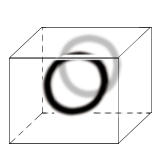
\includegraphics[width=4cm]{inudos/cubo1.png}
  	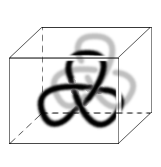
\includegraphics[width=4cm]{inudos/cubo2.png} 
  	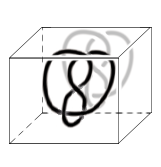
\includegraphics[width=4cm]{inudos/cubo3.png}
  	\centering
  	\caption{De izquierda a derecha: nudo trivial, nudo trébol, nudo de ocho.}
  	\label{trid} 
  \end{figure}

Nos interesa saber cuándo dos nudos son equivalentes: se puede pasar de uno a otro mediante deformaciones. Veámoslo formalmente:\\

Se dice que dos nudos son equivalentes si existe un homeomorfismo de  $\mathds{R}^{3}$ que nos lleve de un nudo al otro. \\


Podemos representar un nudo en el plano visualizando su proyección. Como hay muchas formas de representar un mismo nudo, podremos tener diferentes proyecciones que representen al mismo nudo. Se pueden ver dos proyecciones distintas de un mismo nudo en la figura \ref{cross1}. Algunos ejemplos básicos de proyecciones son los siguientes:\\
  \begin{figure}[h!]
  	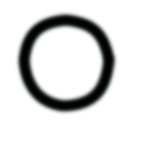
\includegraphics[width=3cm]{inudos/1.jpg}
  	
\includegraphics[width=3cm]{inudos/3f.png} 
  	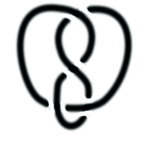
\includegraphics[width=3cm]{inudos/fig8.jpg}
  	\centering
  	\caption{Proyecciones del nudo trivial, nudo trébol, nudo de ocho.}
  	\label{uno} 
  \end{figure}
  
  Podemos ver en ellos una serie de cruces. En concreto en el nudo trébol tenemos 3 cruces y el nudo de ocho tenemos 4 cruces. El nudo trivial destaca porque puede tener proyecciones sin ningún cruce. No obstante, hay nudos con cruces que corresponden a proyecciones del nudo trivial. \\
  
    \underline{\textbf{Definición:}}\\
     Un \textbf{enlace} es una o más curvas cerradas disjuntas en $\mathds{R}^{3}$. Cada una de sus curvas recibe el nombre de componente.\\
     Por ejemplo, el siguiente enlace tiene dos componentes:
  \begin{figure}[h!]
  	
\includegraphics[width=2.7cm]{inudos/enlace.png}
  	\centering
  	\label{dos} 
  \end{figure}

    Por tanto, podemos ver un nudo como un caso particular de enlace en el que sólo tenemos una componente.\\
    
  Una de las cuestiones más interesantes en la teoría de nudos es la siguiente: \\
  ¿Dada un nudo, o alguna proyección suya, podremos saber si se trata del nudo trivial?. A lo largo de este proyecto trataremos de dar respuesta, en parte, a dicha cuestión.\\
  